% !TeX program = XeLaTeX
\documentclass[zihao=5,a4paper]{ctexart}
\ctexset{section/name={第,节},section/format+=\raggedright}
\renewcommand\sectionmark[1]{%
  \markright{\CTEXifname{\textnormal{\textsf{\CTEXthesection}}\quad}{}\textnormal{\textsf{#1}}}}
\usepackage{mathtools}
\usepackage{amssymb}
\usepackage{bm}
\usepackage[width=378bp]{geometry}
\usepackage{zhlineskip}
\SetTextEnvironmentSinglespace{1.25}
\usepackage{caption}
\newlength\prezhcolonhspace
\setlength\prezhcolonhspace{31.5bp}
\makeatletter
\settowidth\@tempdima{图~3:}
\addtolength\prezhcolonhspace{-\@tempdima}
\makeatother
\DeclareCaptionLabelSeparator{zhcolon}{\kern\prezhcolonhspace:}
\captionsetup{labelsep=zhcolon,format=hang}
\usepackage[inline]{enumitem}
\usepackage{booktabs}
\usepackage{hyperref}
\hypersetup{
  colorlinks=true,
  pdfstartview={FitH},
  unicode=true,
  pdftitle={zhlineskip-man},
  pdfauthor={张瑞熹},
}
\usepackage[open,openlevel=-1,numbered]{bookmark}

\makeatletter
% From `doc.dtx'
\ifx\l@nohyphenation\undefined
  \newlanguage\l@nohyphenation
\fi
\newcommand*\meta{}
\DeclareRobustCommand\meta[1]{%
     \ensuremath\langle
     \ifmmode \expandafter \nfss@text \fi
     {%
      \meta@font@select
      \edef\meta@hyphen@restore
        {\hyphenchar\the\font\the\hyphenchar\font}%
      \hyphenchar\font\m@ne
      \language\l@nohyphenation
      #1\/%
      \meta@hyphen@restore
     }\ensuremath\rangle
}
\def\meta@font@select{\itshape}
% From `ltxdoc.dtx'
\newcommand*\cmd[1]{\cs{\expandafter\cmd@to@cs\string#1}}
\def\cmd@to@cs#1#2{\char\number`#2\relax}
\newcommand*\cs{}
\DeclareRobustCommand\cs[1]{\texttt{\char`\\#1}}
\newcommand\marg[1]{%
  {\ttfamily\char`\{}\meta{#1}{\ttfamily\char`\}}}
\newcommand\oarg[1]{%
  {\ttfamily[}\meta{#1}{\ttfamily]}}
\newcommand\parg[1]{%
  {\ttfamily(}\meta{#1}{\ttfamily)}}
% My commands
\newcommand\cls[1]{{\normalfont\ttfamily#1}}
\newcommand\pkg[1]{{\normalfont\ttfamily#1}}
\newcommand\opt[1]{{\normalfont\ttfamily#1}}
\newcommand\env[1]{{\normalfont\ttfamily#1}}
\newcommand*\packagedependency[1]{%
  \mbox{\pkg{#1}~宏包:}}
\newcommand*\keyvaluedescription[2]{%
  \mbox{\texttt{#1} \meta{#2}}}
\newcommand*\fontandsinglespacingratio[2]{%
  #1 & \texttt{#2}}
\newcommand*\defaultleadingratio[3]{%
  \opt{#1} & \texttt{#2} & \texttt{#3}}
\newenvironment{originalpmatrix}{\left(\env@matrix}{\endmatrix\right)}
\newenvironment{originalcases}{\env@cases}{\endarray\right.}
\makeatother

\title{\vspace*{-18bp}\pkg{zhlineskip} 宏包}
\author{张瑞熹\thanks{\href{mailto:ruixizhang42@gmail.com}{\nolinkurl{ruixizhang42@gmail.com}}。}}
\date{2018~年 10~月 12~日}

\begin{document}

\maketitle

\tableofcontents

\section{简介}

在西文排版里,相邻两行\emph{基线}(baseline)之间的距离称为\emph{行距}(leading,
发音为 ledding)。这个词的词根是 lead,即\emph{铅}。早在铅字时代,每当工匠填满
一行铅字之后要开始填下一行,都会在两行之间插入铅条,从而适当扩大行距。因为西文的
每个字母四周与其\emph{字框}(em-box,见图~\ref{fig:eng-font-size})间有
较大的空隙,所以一般不需要插入很高的铅条。一般来说,西文的行距为\emph{字号}(font
size)的 $1.2$ 至 $1.45$~倍\footnote{参见
\url{https://practicaltypography.com/line-spacing.html}。}。

\begin{figure}[h]
\centering

\includegraphics{Latinmetrics}
\caption[西文字体]{西文字体。绿色方框即为 em-box,它在纸上的实际边长就是西文字号。}
\label{fig:eng-font-size}
\end{figure}

中文排版虽然没有基线的概念,但有非常相似的概念:\emph{底线}(ideographic baseline,
见图~\ref{fig:chi-font-size})。中文里相邻两行底线之间的距离,与西文里行距的
概念是一致的。另一概念是上一行底线和下一行\emph{顶线}之间的距离,即\emph{行间距}(line
gap),这与西文里插入铅条的高度是一致的。由于汉字四周与其字框间的空隙较小,所以需要
使用比西文更大的行间距。根据场合不同,行间距从字号的 $1/4$ 至 $1$~倍不等:以中文
书刊为例,行间距一般为字号的 $1/2$ 至 $2/3$~倍\footnote{参见张胜涛、王忆波著
《方正飞腾4.0实用培训教程》,第~6.1.1~节。},即行距约为字号的 $1.5$ 至 $1.67$~倍。

\begin{figure}[h]
\centering
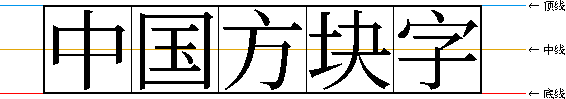
\includegraphics{CJKmetrics}
\caption[中文字体]{中文字体。汉字字面几乎占满整个字框,字框的边长即为中文字号。}
\label{fig:chi-font-size}
\end{figure}

在一般情况下,\CTeX 会默认地用 \opt{linespread=1.3} 这个文档类选项将中文的
行距设置为字号的 $1.56$~倍(基础行距是字号的 $1.2$~倍,而 $1.2 \times 1.3
= 1.56$)。通过这种方法扩大全文的行距,自然会影响到文章里数学公式的行距。数学公式
主要是由西文字符构成的,把它们按照中文的行距进行排版,就会显得有些松散。
图~\ref{fig:math-leading} 的左边是 \CTeX 默认设置的排版效果,而右边则是
配合使用 \pkg{zhlineskip} 宏包的排版效果。\pkg{zhlineskip} 宏包还允许
用户自定义数学行距的大小。

\begin{figure}[h]
\sbox0{%
\begin{minipage}[t]{162pt}
\fontsize{9}{10.8}\linespread{1.3}\selectfont
\rule{0pt}{\ht\strutbox}\hspace{2\ccwd}%
设 $\bm{I}_2=\begin{psmallmatrix} 1&0\\0&1 \end{psmallmatrix}$.
又设 $\bm{A}=(a_{ij})_{m \times n}$ 为 $m$~行 $n$~列的实值矩阵, 即
\[
\bm{A} = \begin{originalpmatrix}
a_{11} & a_{12} & \dotsc & a_{1n} \\
a_{21} & a_{22} & \dotsc & a_{2n} \\
\vdots & \vdots &        & \vdots \\
a_{m1} & a_{m2} & \dotsc & a_{mn} \\
\end{originalpmatrix}.
\]
其中, $a_{ij} \in \mathbb{R}$, $i=1,\dotsc,m$, $j=1,\dotsc,n$.
因为
\[
\sum_{\substack{i=1\\i\neq j}}^m a_{ij} = \begin{originalcases}
0, & j=1,\\
1, & j>1,\\
\end{originalcases}
\]
我们得到……\rule[-\dp\strutbox]{0pt}{\dp\strutbox}
\end{minipage}%
}%
\centering
\rule[\dimexpr-\dp0-0.5em\relax]{0.4pt}{\dimexpr\dp0+\ht0+1em\relax}\quad
\copy0\quad
\rule[\dimexpr-\dp0-0.5em\relax]{0.4pt}{\dimexpr\dp0+\ht0+1em\relax}\quad
\begin{minipage}[t]{162pt}
\fontsize{9}{10.8}\linespread{1.25}\selectfont
\hspace{2\ccwd}%
设 $\bm{I}_2=\begin{psmallmatrix} 1&0\\0&1 \end{psmallmatrix}$.
又设 $\bm{A}=(a_{ij})_{m \times n}$ 为 $m$~行 $n$~列的实值矩阵, 即
\[
\bm{A} = \begin{pmatrix}
a_{11} & a_{12} & \dotsc & a_{1n} \\
a_{21} & a_{22} & \dotsc & a_{2n} \\
\vdots & \vdots &        & \vdots \\
a_{m1} & a_{m2} & \dotsc & a_{mn} \\
\end{pmatrix}.
\]
其中, $a_{ij} \in \mathbb{R}$, $i=1,\dotsc,m$, $j=1,\dotsc,n$.
因为
\[
\sum_{\substack{i=1\\i\neq j}}^m a_{ij} = \begin{cases}
0, & j=1,\\
1, & j>1,\\
\end{cases}
\]
我们得到……
\end{minipage}\quad
\rule[\dimexpr-\dp0-0.5em\relax]{0.4pt}{\dimexpr\dp0+\ht0+1em\relax}%
\llap{\rule[\dimexpr-\dp0-0.5em\relax]{\dimexpr2\wd0+4em+1.2pt\relax}{0.4pt}}%
\llap{\rule[\dimexpr\ht0+0.5em-0.4pt\relax]{\dimexpr2\wd0+4em+1.2pt\relax}{0.4pt}}
\caption[数学行距对比]{数学行距对比。在左图中,大矩阵 \env{pmatrix} 与分类
  \env{cases} 环境受到了影响,行距都被扩大了;但第一行文本里的小矩阵与末尾公式
  里求和号的下角标却没有受到影响,行距仍然较为紧凑。在右图中,数学公式的行距都是
  西文的行距,格式比较统一,行间公式里的大括弧、大括号也不会特别突兀。}
\label{fig:math-leading}
\end{figure}

综上所述,在进行中西文混排时,最好能够区分中文与西文的行距。在使用 \pkg{zhlineskip}
时,就可以分开处理中文文本与数学公式的行距。用户甚至还能分别指定正文行距与脚注
行距,实现灵活的排版。同时,\pkg{zhlineskip} 宏包能够恢复各种“多行”数学环境
(包括矩阵、分类、多行公式推导等等)的行距,使数学行距符合西文行距的规范。

最后,\pkg{zhlineskip} 宏包还支持用户在一定范围内按 Microsoft Word 的
“多倍行距”进行排版\footnote{我在这里还假定“被要求”用的字体是中易系列字体,
这包括中易宋体、中易黑体、中易楷体与中易仿宋。参见第~\ref{sec:MS-Word}~节。}。
用户可以指定“多倍行距”的倍数,但是这个支持只保证用 \TeX 排版出来的文本行距
与用 Microsoft Word 的行距相同。硬要用 \TeX 模仿 Microsoft Word 是没有
太大意义的。

\subsection{宏包依赖}

本宏包是在 \CTeX 宏集大环境下设计出来的,目的是要分开处理中文与数学的行距。
如果你没用 \CTeX 的文档类,那么不建议使用本宏包。\pkg{zhlineskip} 依赖于
下面这些宏包:
\begin{itemize}[noitemsep]
\item \packagedependency{kvoptions}为用户提供载入本宏包的键值选项。
\item \packagedependency{xintexpr~}实现精确的浮点运算。
\item \packagedependency{etoolbox~}处理脚注行距与数学行距时需要打补丁。
\item \packagedependency{mathtools}只有在恢复数学行距为西文行距时,才会载入这个宏包。
\end{itemize}
请确保你的 \TeX 套装里已经安装好了以上这些宏包的最新版本。

\section{功能介绍}

首先,请避免使用“多倍行距”这个概念:Microsoft Word 中“单倍行距”的值严重依赖于
字体(参见第~\ref{sec:MS-Word}~节)。在严格的排版中,一般都会给定具体的字号与
行距,如 $12$~磅的字号、$22$~磅的行距。对于一般的用户,指定目标行距相比字号的
倍数即可。\pkg{zhlineskip} 宏包可以自动提取基础行距(即 \TeX 中的单倍行距)
相比字号的倍数(详见表~\ref{tab:default-leading-ratio}),再通过用户指定的
倍数来计算所需的行伸展因子。
\begin{table}[h]
\centering
\caption[基础行距倍数]{\cls{ctexart} 与 \cls{article} 各个文档类选项
  设置的基础行距倍数。}
\label{tab:default-leading-ratio}
\begin{tabular}{l l l}
\toprule
文档类选项 & 正文基础行距 & 脚注基础行距 \\
\midrule
\defaultleadingratio{zihao=5}{1.2}{1.2} \\
\defaultleadingratio{zihao=-4}{1.2}{1.2} \\
\defaultleadingratio{10pt}{12/10}{9.5/8} \\
\defaultleadingratio{11pt}{13.6/10.95}{11/9} \\
\defaultleadingratio{12pt}{14.5/12}{12/10} \\
\bottomrule
\end{tabular}
\end{table}

\subsection{宏包载入时的键值选项}

载入 \pkg{zhlineskip} 宏包时可以设定五个基本的键值选项,它们分别是:
\begin{description}
\item[\keyvaluedescription{bodytextleadingratio}{real}]
指定正文目标行距相比于正文字号的倍数。以书刊为例,建议设置在~$1.5$ 至~$1.67$
之间。缺省值是~\opt{1.5},即 $1/2$~的行间距。
\item[\keyvaluedescription{footnoteleadingratio}{real}]
指定脚注目标行距相比于脚注字号的倍数,它可以比正文的倍数稍小一些,建议设置在正文
倍数的 $98\%$ 至 $100\%$ 之间。缺省值是~\opt{1.48},即大约为正文倍数的~$98.67\%$。
\item[\keyvaluedescription{restoremathleading}{boolean}]
指定是否将数学公式的行距恢复成西文基础行距。缺省值是~\opt{true},即恢复数学
行距。该选项为~\opt{true} 时,会自动载入 \pkg{mathtools} 宏包,此时还可以
利用 \cmd{\SetMathEnvironmentSinglespace}\marg{real} 命令\emph{微调}
数学公式的基础行距。
\item[\keyvaluedescription{UseMicrosoftWordMultipleLineSpacingWithSimSunHeiKaiFangFonts}{boolean}]
如果大学论文要求正文使用中易字体,还要求使用 Microsoft Word 的“多倍行距”,
那么用户可以将该选项设置为~\opt{true},并通过 \opt{MSLineSpacingMultiple}
选项指定“倍数”,这会忽略用户之前指定的正文与脚注行距倍数,但与数学行距的设置独立。
该选项的缺省值是~\opt{false}。
\item[\keyvaluedescription{MSLineSpacingMultiple}{real}]
设置 Microsoft Word“多倍行距”的“倍数”,在
\opt{UseMicrosoftWordMultipleLineSpacingWithSimSunHeiKaiFangFonts\!}
为真时才生效。缺省值是~\opt{1.15},与 Microsoft Word 缺省值一致。
对于中易字体,这相当于设置了目标行距为字号的 $1.49140625$~倍
(参见第~\ref{sec:MS-Word}~节)。
\end{description}

\subsection{宏包载入后的用户命令}

\subsubsection{调整数学公式的行距}

当键值选项 \opt{restoremathleading} 为真时,数学公式的行距被恢复成字号的
$1.2$~倍。对于某些字面较大的数学字体(例如类似 Palatino 的字体),这个基础行距
会显得过小。此时,用户可以通过如下命令微调数学行距:
\begin{description}
\item[\cmd{\SetMathEnvironmentSinglespace}\marg{real}]
如果数学字体是 \pkg{newpxmath} 或 TeX Gyre Pagella Math,那么数学行距
在字号 $1.2$~倍的基础上再扩大 $1.05$~倍更加合适。此时只需指定
\verb|\SetMathEnvironmentSinglespace{1.05}| 即可。
\end{description}
本宏包恢复的多行数学环境包括:
\begin{description}
\linespread{1.05}\selectfont
\raggedright
\item[\LaTeX 环境]
\env{array};
\item[\pkg{amsmath} 宏包各环境]
\env{matrix},
\env{pmatrix},
\env{bmatrix},
\env{Bmatrix},
\env{vmatrix},
\env{Vmatrix},
\env{cases},
\env{aligned},
\env{alignedat},
\env{gathered},
\env{gather},
\env{gather*},
\env{alignat},
\env{alignat*},
\env{xalignat},
\env{xalignat*},
\env{xxalignat},
\env{align},
\env{align*},
\env{flalign},
\env{flalign*},
\env{multline},
\env{multline*},
\env{split};
\item[\pkg{mathtools} 宏包各环境]
\env{matrix*},
\env{pmatrix*},
\env{bmatrix*},
\env{Bmatrix*},
\env{vmatrix*},
\env{Vmatrix*},
\env{cases*},
\env{dcases},
\env{dcases*},
\env{rcases},
\env{rcases*},
\env{drcases},
\env{drcases*},
\env{multlined},
\env{lgathered},
\env{rgathered}。
\end{description}
超出上述列表范围、用户自定义的\emph{数学}环境,可用如下命令恢复其行距:
\begin{description}
\item[\cmd{\RestoreMathEnvironmentLeading}\marg{env name}]
本宏包恢复数学环境 \env{pmatrix} 行距,通过
\verb|\RestoreMathEnvironmentLeading{pmatrix}| 实现。
\end{description}

\subsubsection{调整西文文本的行距}

与数学行距命令对应,本宏包还提供两个调整\emph{西文文本}行距的命令,用法类似。
\begin{description}
\item[\cmd{\SetTextEnvironmentSinglespace}\marg{real}]
如果西文字体是 \pkg{newpxtext} 或 TeX Gyre Pagella,那么可以用
\verb|\SetTextEnvironmentSinglespace{1.05}|。
\end{description}
本宏包恢复的多行\emph{文本}环境包括:
\begin{description}
\linespread{1.05}\selectfont
\raggedright
\item[\LaTeX 环境]
\env{tabular}。
\end{description}
其它\emph{文本}环境,可用如下命令恢复其行距:
\begin{description}
\item[\cmd{\RestoreTextEnvironmentLeading}\marg{env name}]
本宏包恢复文本环境 \env{tabular} 行距,通过
\verb|\RestoreTextEnvironmentLeading{tabular}| 实现。
\end{description}

如果作者没有顾及到某些\emph{基本环境},鼓励用户向 \pkg{zhlineskip} 宏包的
\href{https://github.com/CTeX-org/ctex-kit/issues}{GitHub 维护页}%
提供相关信息。

\subsection{使用范例}

下面以 \CTeX 提供的 \cls{ctexart} 文档类为例,展示 \pkg{zhlineskip} 的
使用方法。

\subsubsection*{例:直接载入}

\begin{verbatim}
    \documentclass{ctexart}
    \usepackage{zhlineskip}
    \begin{document}
    正文测试。
    \end{document}
\end{verbatim}

\subsubsection*{\boldmath 例:指定正文行距为字号的 $1.6$~倍}

\begin{verbatim}
    \documentclass{ctexart}
    \usepackage[
        bodytextleadingratio=1.6, %  设置正文行距倍数为 1.6
        footnoteleadingratio=1.57 %  设置脚注行距倍数为 1.57
      ]{zhlineskip}               %  缺省数学行距倍数为 1.2
    \begin{document}
    正文测试。
    \end{document}
\end{verbatim}

\subsubsection*{\boldmath 例:按照 Microsoft Word 设置“$1.62$~倍行距”}

\begin{verbatim}
    \documentclass{ctexart}
    \usepackage[
        restoremathleading=false,
        UseMicrosoftWordMultipleLineSpacingWithSimSunHeiKaiFangFonts,
        MSLineSpacingMultiple=1.62
      ]{zhlineskip}
    \begin{document}
    按照 Microsoft Word 设置 1.62~倍行距。
    \end{document}
\end{verbatim}

\subsubsection*{例:中文正文里需要插入成段的西文}

如果插入的西文是引用参考文献的段落,那么用 \env{quote} 或者 \env{quotation}
环境比较合适。此时可以在引用环境内部使用 \cmd{\linespread} 命令。建议将必选
参数设置在正文行距倍数的 $0.7$~倍左右。例如,在载入 \pkg{zhlineskip} 宏包后,
如果正文行距为字号的 $1.5$~倍,那么使用
\verb|\linespread{1.05}\selectfont| 就比较合适。
\begin{verbatim}
    \documentclass{ctexart}
    \usepackage{zhlineskip}
    \begin{document}
    下面引用一段出自英文文献的段落:
    \begin{quotation}
    \linespread{1.05}\selectfont% 此处数值为正文行距倍数的 0.7 倍左右
    A quotation from English literature. 
    \end{quotation}
    \end{document}
\end{verbatim}
当然,在这个例子里使用 \verb|\linespread{1}\selectfont| 也是可以的。

\subsection{Microsoft Word 中的“单倍行距”}
\label{sec:MS-Word}

Microsoft Word 中“单倍行距”的设置,其行距相比于字号的倍数严重依赖于字体。
表~\ref{tab:word-line-height} 列出几种常用字体对应的倍数。正是因为“单倍
行距”本身随着字体而变化,所以请尽量避免使用“多倍行距”的概念!
\begin{table}[h]
\centering
\caption[单倍行距倍数]{在 Microsoft Word 中设置“单倍行距”后,实际的行距依赖于字体。}
\label{tab:word-line-height}
\begin{tabular}{l l}
\toprule
字体名称 & 单倍行距除以字号的倍数 \\
\midrule
\fontandsinglespacingratio{Arial}{2355/2048~=~1.14990234375} \\
\fontandsinglespacingratio{Times New Roman}{2355/2048~=~1.14990234375} \\
\fontandsinglespacingratio{中易系列字体}{~332/256~~=~1.296875} \\
\fontandsinglespacingratio{思源黑体}{1924/1000~=~1.924} \\
\fontandsinglespacingratio{思源宋体}{1869/1000~=~1.869} \\
\bottomrule
\end{tabular}
\end{table}

%\section{代码实现}

\end{document}
